% !TEX root = ../thesis_main.tex



%%%% --- * --- %%%%
\clearpage	
\chapter{Estimating Systematic Effects}
\label{systematics_chapter}
\note[color=org]{Do I want this chapter combined with the analysis chapter?  If that chapter includes all the stuff about G4, it's going to be unwieldy and huge.}
%\note{How do I even \emph{do} these estimations?}

\section{Overview}	
A summary of systematics goes here.  In words, yes, but also in table form.


% !TEX root = ../thesis_main.tex



%%%% --- * --- %%%%	
%\renewcommand{\arraystretch}{1.6}

\begin{table}[h!!!!t]
	\begin{center}
	\begin{tabular}{ l  c  c  }
		\multicolumn{1}{l}{ Source} 		& \multicolumn{2}{c}{ \;\;\; \;\;\; Uncertainty \;\;\; \;\;\; }   
		\\
		\multicolumn{1}{l}{ } 				& \multicolumn{1}{c}{\;\; $\bFierz$}   & \multicolumn{1}{c}{$\Abeta$}   	
		\\  \hline
		%%% % %%%
		Scintillator Calibration 			& 0.003								& 0.0003											
		\\
		Scintillator Threshold  			& 0.004 							& 0.0004 						
		\\
		%%% % %%%
		DSSD Individual Strip SNR 			& 0.006								& 0.0007													
		\\
		DSSD Energy Agreement	  			& 0.005 							& 0.0006 						
		\\
		DSSD Detection Radius	  			& 0.006 							& 0.0017 						
		\\
		DSSD Energy Threshold	  			& 0.005 							& 0.0005 						
		\\
		%%% % %%%
		Atomic Cloud			  			& 0.002 							& 0.0002 						
		\\
		%%% % %%%
		Background				  			& 0.004 							& 0.0003 						
		\\
		%%% % %%%
		Beta Scattering				  		& 0.031 							& 0.0025 						
		\\
		%%% % %%%
		Low Energy Tail				  		& 0.008 							& 0.0007 						
		\\
		%%% % %%%
		Mirror Thickness				  	& 0.013 							& 0.0017 						
		\\
		DSSD Thickness				 	 	& 0.013 							& 0.0017 						
		\\
		Beryllium Foil Thickness			& 0.004								& $\!\!\!\!\!\! < 0.0001$ 			
	%	\\
		%%% % %%%
		\\  \hline
		\multicolumn{1}{l}{ Total Systematics} & \multicolumn{1}{c}{0.039}  & \multicolumn{1}{c}{0.0041}
%		Total Systematics			  		& 0.056 							& 0.0055 						
		\\
		\multicolumn{1}{l}{ Statistics} 	   & \multicolumn{1}{c}{0.084}  & \multicolumn{1}{c}{0.0082}
%		Statistics				  			& 0.084 							& 0.0082 						
	%	\\  \hline
		%%% % %%%
	\end{tabular}
	\end{center}
	\caption[Error Budget]{Error budget for the two-parameter analysis for $\bFierz$ and $\Abeta$, with all data included.  All uncertainties are believed to be uncorrelated, and are added in quadrature.  Final results: 
	$\mbox{ $\bFierz = 0.033 \pm 0.084(\textrm{stat}) \pm 0.039(\textrm{sys})$ }$ and $\mbox{ $\Abeta = -0.5738 \pm 0.0082(\textrm{stat}) \pm 0.0041(\textrm{sys})$ }$. }
	\label{table:budget}
\end{table}

%\renewcommand{\arraystretch}{1}





%	\section{Low-energy Scintillator Threshold}
%	%\\*
	Choice of low-energy scintillator threshold has a large systematic effect...  \aside{It's actually not nearly as big as I'd originally expected.  It's huge in the lineshape thing, but pretty tiny in everything else.}


	\note[color=jb]{from John:  ``I used Ben's threshold when determining the uncertainty from the lineshape tail (UFTLT). 
If you're saying the UFTLT depends on the threshold used, ok, of course it does. But if you're claimiing that UFTLT depends on the **uncertainty** of the threshold, that's manifestly smaller than the UFTLT itself, and I'm going to assert it isn't worth evaluating.''}
	
	\section{BB1 Radius, Energy Threshold, Agreement}
	\label{section:bb1_systematics}
	%\\*
	BB1 radius cut can help to eliminate scattered events.  Energy threshold selection and statistical agreement between BB1 detectors' energies only makes a small effect on results.  BB1 radius itself has a pretty big effect on the result, but we can at least just G4 it away.  The remaining systematic effect is pretty small.  
	\note[color=jb]{JB:  I hope the discussion is clear in your head.  Any effect that relies on scattering computation in G4 should have an uncertainty on order 10\% of the correction -- hopefully you are keeping a distinction here between the finite geometry acceptance (which I guess is exact) scattering off the collimator.}
	\note[color=jb]{As per JB's comment in section~\ref{thesisconventionjb}:   ``statistical agreement between BB1 X and Y detectors' energies only makes a small effect on results" does not need the technical details beyond that statement."}
	
\missingfigure{Surely this requires at *least* one image of the pixelated BB1 data.  Maybe some of a few waveforms and energy distributions too.  ....Feels like cheating to include some of that stuff, since Ben was the one who actually used it mostly.}
\note[color=jb]{JB on missing figure:  ``if you used such an image as part of your uncertainty estimate, yes [include it]''}

\note{Remember:  There's noise applied to simulated BB1s, matching some spectrum.}
In the end, we get our results from the scintillator energy only, without summing the BB1 energy back in.  Energy absorbed in DSSDs is only used as (a) a tag for events, and (b) contributing to the total beta energy loss before the beta arrives at the scintillator.
\note[color=jb]{JB:  The simulations of course include it event-by-event, not just a minimally ionizing average loss.}

\section{Background Modeling -- Decay from Surfaces within the Chamber}
	So many surfaces, all of which can get stray 37K atoms stuck to them.  Then they decay from a place that isn't the actual trap center, and it contaminates our stuff.
	
%	\missingfigure{Show modelled TOF spectra in comparison with real TOF spectra.  Show the cut we made on that. }
	\note[color=jb]{JB on figures that might go here:  Figure 6.4 (currently that picture of the TOF spectrum) could either be here, or you could reference it from here. The TOF histogram is a great start. Adding the asymmetry[TOF] indeed would be vital.}
	\missingfigure{Show the "average asymmetry" (all energies) as a function of TOF, with real data, best model normalization, and extrema of model normalizations.  Show our cut.  Turns out, it's a lot of work for a really tiny correction.  Oh well.}
	\note[color=jb]{JB on the *actual* figure I had been planning to put here, and my remarks about it:  Indeed it will be critical to show a clear compelling version of this figure in thesis and in a paper.  It was vital to minimize and determine this background to avoid fitting a polynomial to it from the wings,  even more so for the energy dependence of A than for its average -- you should say so.
	\\ ... \\
The reason the correction is small is because of all your hard work.}
	
	We model the beta TOF from the surfaces in G4, event by event.  This is necessary because scattered \aside[color=jb]{JB:  ``I wouldn't call these "scattered" events... that's very misleading.'' 
	\\ ... \\ 
	Yeah, I should really stop doing that.  
	\\ ... \\ 
	Wait no, scattered is what I mean!  But fine, my phrasing is really unclear.} events will have their TOF changed to account for a longer beta pathlength, and we're preferrentially cutting away the events that don't have a TOF in the appropriate range.  ....And then have COMSOL generate electron TOFs for SOEs starting from the start points picked by G4.  Ran COMSOL for 0 eV SOEs, and again for Levinger spectrum SOEs.  Used ~9\% 0eV SOEs in the end.  I forget which Levinger distribution I used in the end.  \aside[color=jb]{JB:  Please comment on whether or not it was important to have this energy distribution.}  The point is, for each event, you've simulated a beta TOF that may or may not be scattered off of something before it hits a detector, and you have a SOE TOF for an event originating at that same point, so you subtract them to model the TOF you'd measure in an experiment.  Also, because you've done the scattering with G4, you get the beta energy corrected for any scattering that happened.  This way, one can estimate %\aside[color=jb]{JB:  `you know precisely' $\rightarrow$ `you can estimate'} 
how many ``bad" events are eliminated with the TOF cut, as well as the fraction of ``bad'' events left in what remains.
	
%	\subsection{Decay from Chamber Surfaces}

\section{Quantifying the Effects Backscatter with Geant4}
	Beta decay (back-)scatter from surfaces within the experimental chamber is a significant systematic, and it must be evaluated, quantified, and corrected for.  This is done via a series of GEANT4 simulations.  While only a small fraction of events are affected, the process results in an energy loss in the beta that can, if not understood, be misinterpreted as the exact signal we're searching for.  It is therefore imperative that this be well understood. 
	\aside{Oh god.  Have I even \emph{tried} to quantify the combined systematic that comes out of the TOF cut?  Do I need to, or is it double-counting?  Ugh, it would be such a headache to do this.  Maybe I can at least do it at the end -- because I might never get my code back to the way it was.}


%	\missingfigure{Show simulated $\cos\theta$ vs TOF.  You can just make a lot of that go away with a properly selected cut.}
\begin{figure}[h!!!t]
	\centering
	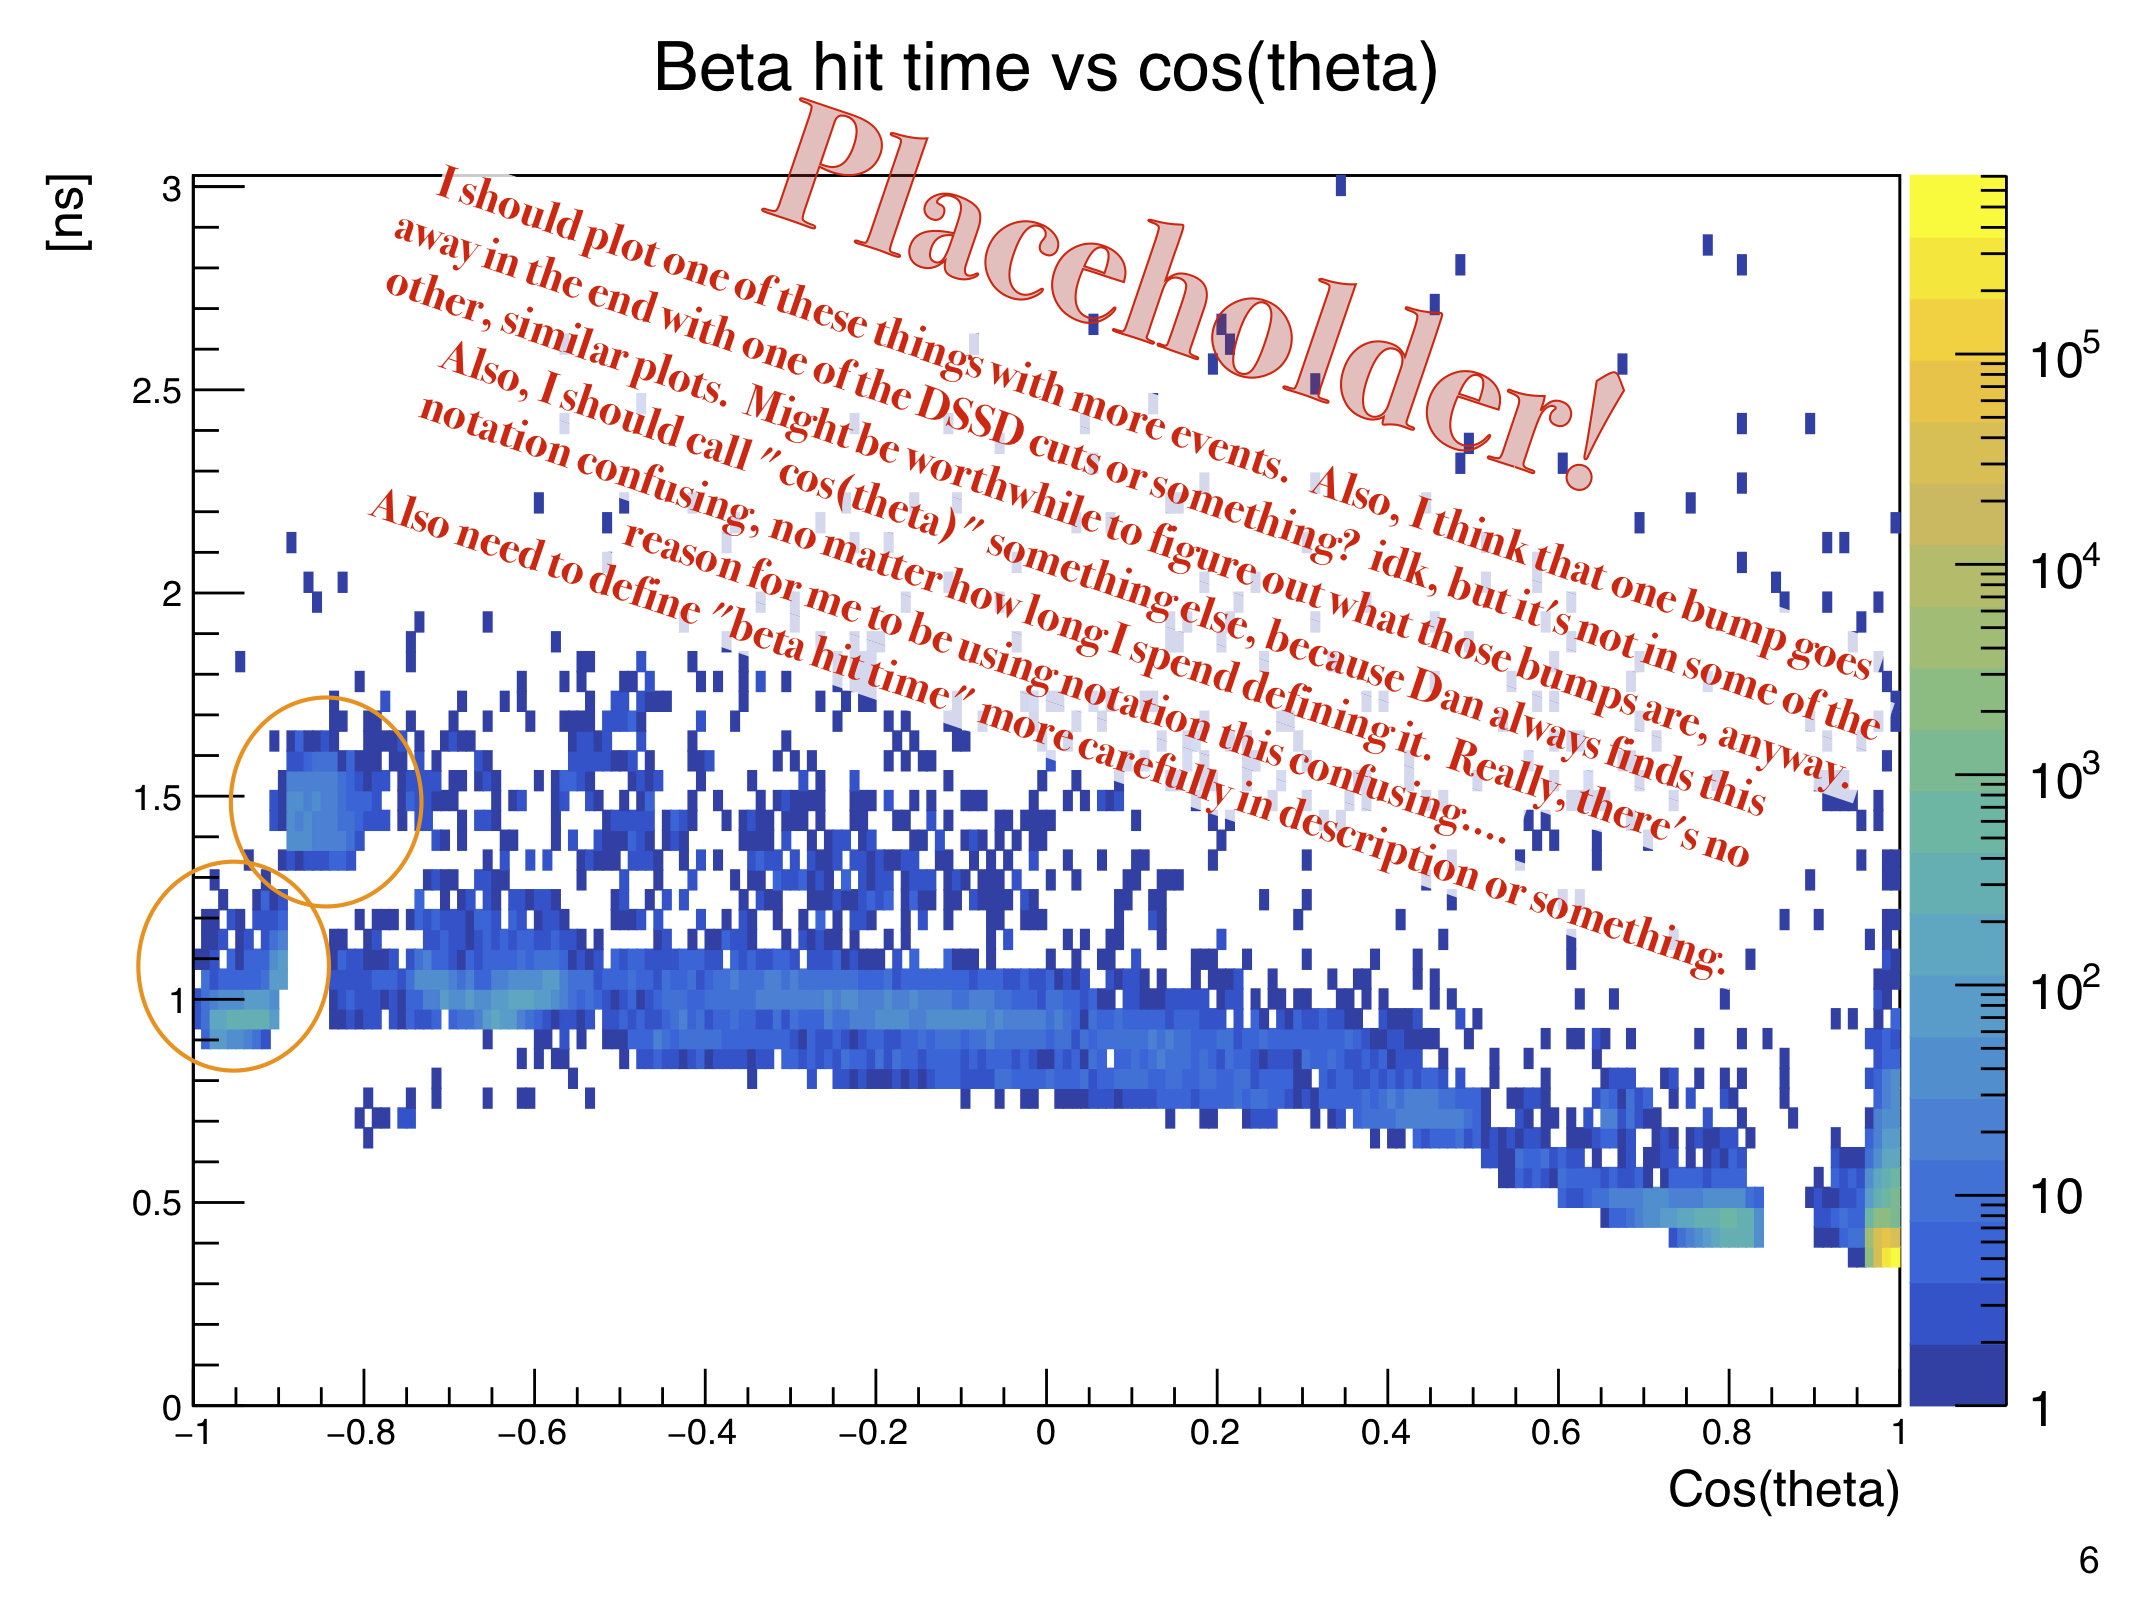
\includegraphics[width=.999\linewidth]
	{Figures/toa_vs_costheta.png}
	\caption[Simulated Beta TOA vs emission angle w.r.t. detector orientation]{Simulated Beta TOA vs emission angle w.r.t. detector orientation}	
	\label{fig:toa_vs_costheta}
\end{figure}
\note[color=jb]{JB says:  
Please discuss this at the next meeting.  (ETA:  Done!)
\\
Indeed this is why you should avoid calling the events originating not from the trap 'scattered events.' More importantly, why it was so critical that you reduced the size of the correction by timing bad events out. I would say you have a well-determined TOF cut to minimize this error-- a cut that could not have been done blind without an unreasonably perfect simulation.  Thus the exact spot of the cut should not be considered to introduce a systematic. }


%%%% --- * --- %%%%
\section{Lineshape Reconstruction}
	\note[color=jb]{This section should reference Clifford.~\cite{clifford}.}
	\subsection{Motivation}
	This process is used because the (back-)scatter, which it itself an important systematic, is largely independent of a wide variety of other experimental effects.  These other effects must all be evaluated, but it is computationally prohibitive to re-evaluate the scattering with every other effect under consideration.
	
	\subsection{What is it and how does it work?}
	Mono-energetic beta decay events are generated in GEANT4, which outputs an energy spectrum for unscattered and forward-scattered beta events in the detector.  These spectra are fit to a function to model the scintillator resolution, as well as energy loss in materials that the beta passed through before arriving at the scintillator.  These spectrum fits are performed for a set of beta energies, and parameters are extrapolated to be applied to betas emitted at intermediate energies.  Thus, the whole spectrum can be modeled.  Pictures will make this clearer. 
	
    \begin{figure}[h!!!t]
    	\centering
    	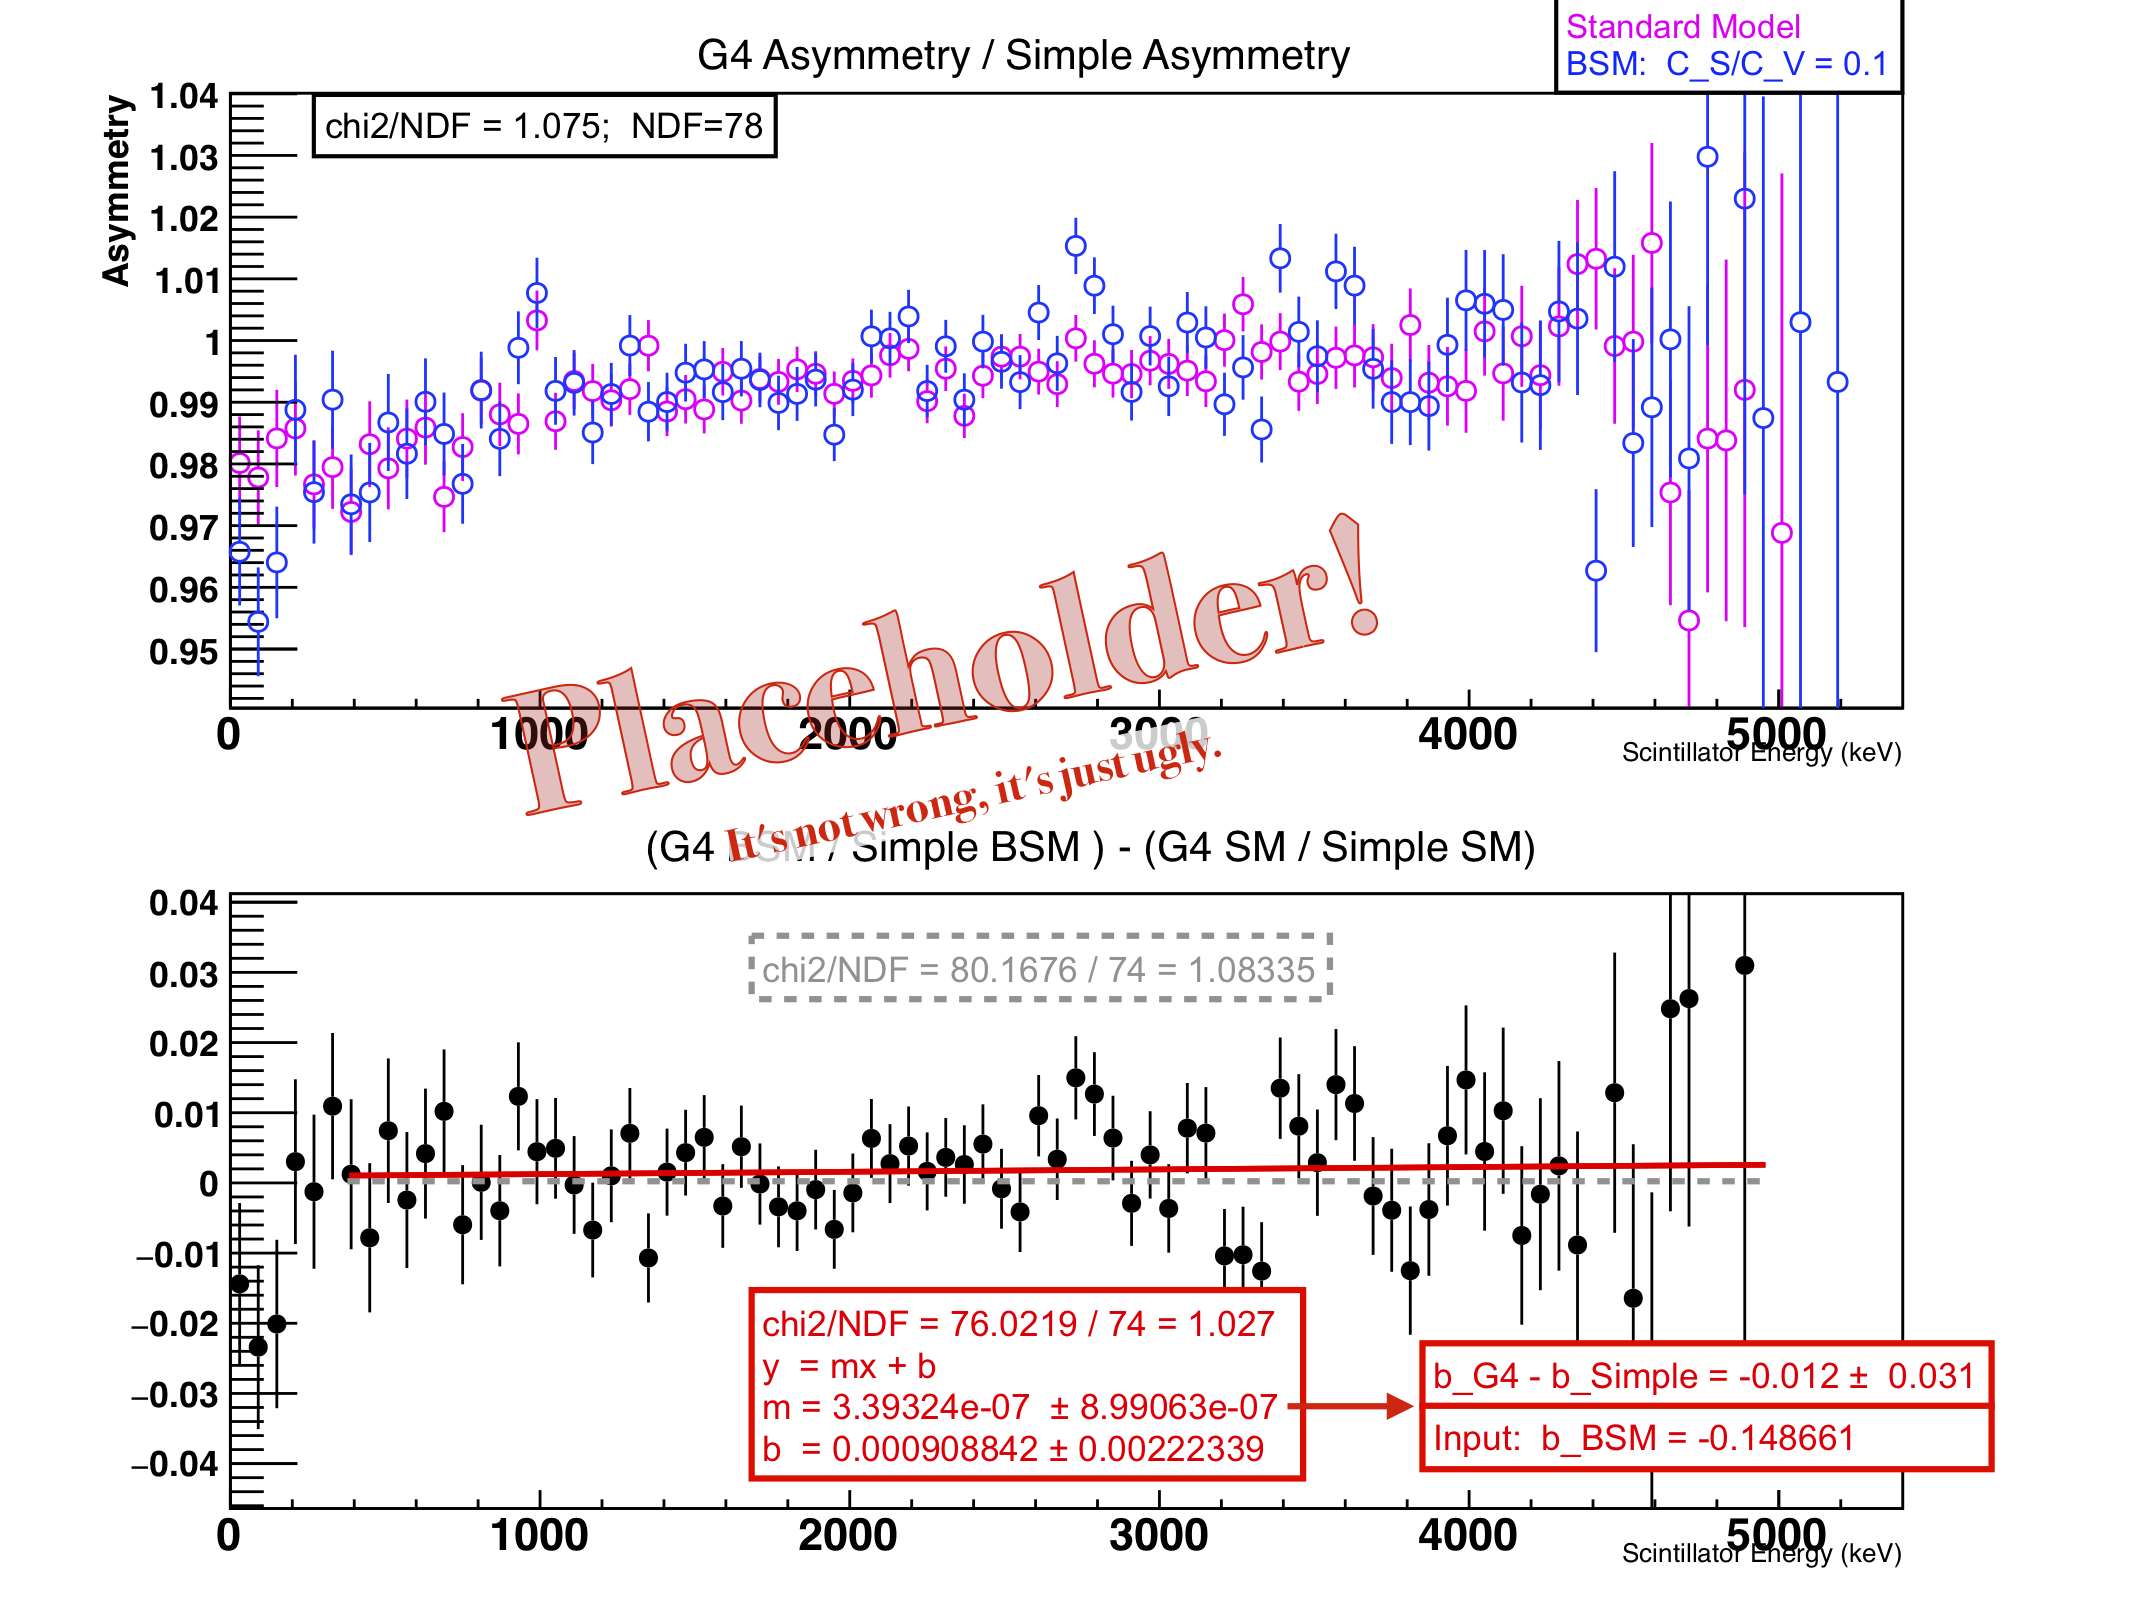
\includegraphics[width=.999\linewidth]
    	{Figures/LineshapeDemo_prelim.png}
    	\caption[Lineshape Comparison]{I'm not actually sure if this picture shows what I want it to.  The point is, if I apply this rough lineshape to stuff that I SimpleMC-ed, then I can evaluate that way various systematic effects that would be time-consuming to actually simulate with G4.  This picture is  *supposed* to be a demonstration that this approach actually works... }	
    	\label{fig:lineshape_demo}
    \end{figure}
	
	\subsection{The Math-Specifics}
	I'll write down the specific functions I'm using, and the parameter values I'm using.  (Maybe this should go in an appendix instead?)  I'll describe the adjustments I make to the spectrum so that it can work even for the dataset where the scintillators' resolutions have changed.
	
	\subsection{The Results -- Things That Got Evaluated This Way}
	As it turns out, only cloud parameters were evaluated this way. \aside[color=jb]{JB:  so it's still critical to write down more of the lineshape work.}
Trap position, size, sail velocity, temperature.  But then we varied the lineshape anyhow, to account for G4 doing a bad job of modelling the bremsstrahlung (sp?).
	%Thicknesses of the SiC mirror, the Be foil, and the DSSD.  Scintillator calibration.  
	\note[color=jb]{JB:  yes, brems strahlung is 'braking radiation' so gets 2 ss's. 
the lineshape tail in any scintillator also includes backscattered events -- we are not claiming the 2-pixel cut is complete}
	
	    \begin{figure}[h!!]
    	\centering
    	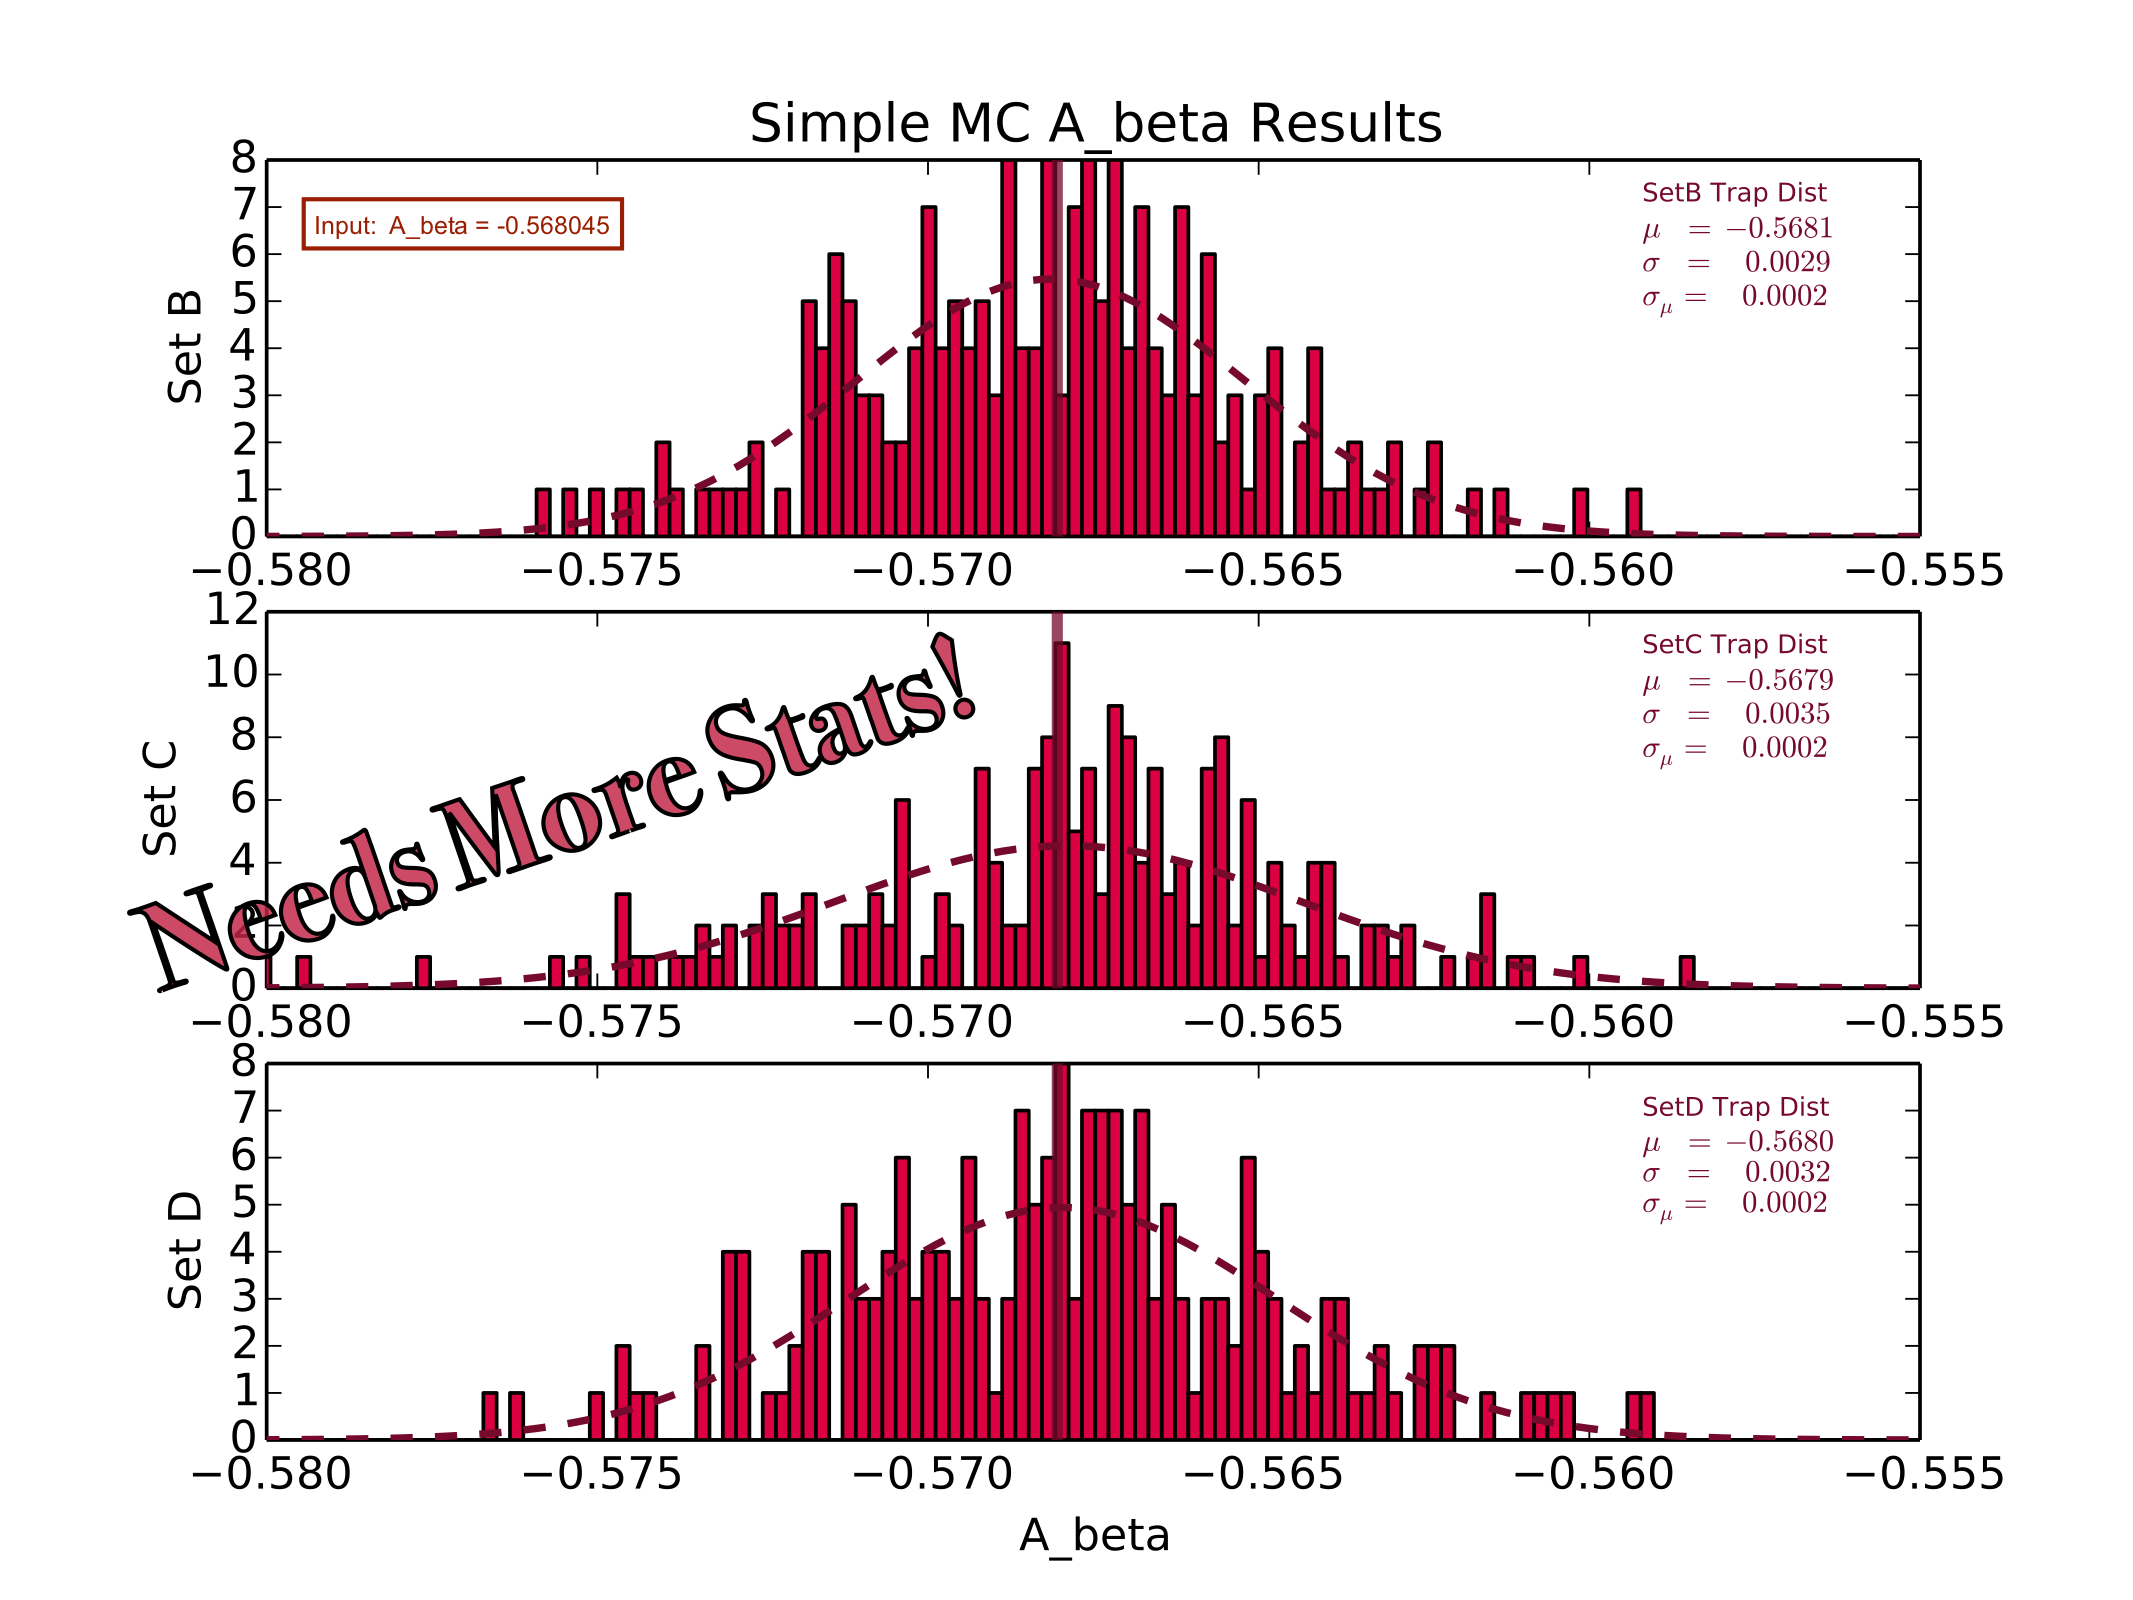
\includegraphics[width=.999\linewidth]
    	{Figures/Position_Err_Abeta_prelim.png}
    	\caption[$\Abeta$ Position Error]{Estimated uncertainty in $\Abeta$ resulting from uncertainty and variation in the cloud parameters.  Evaluated by the lineshape reconstruction method.}	
    	\label{fig:Abeta_position_err}
		\end{figure}

	    \begin{figure}[h!!]
    	\centering
    	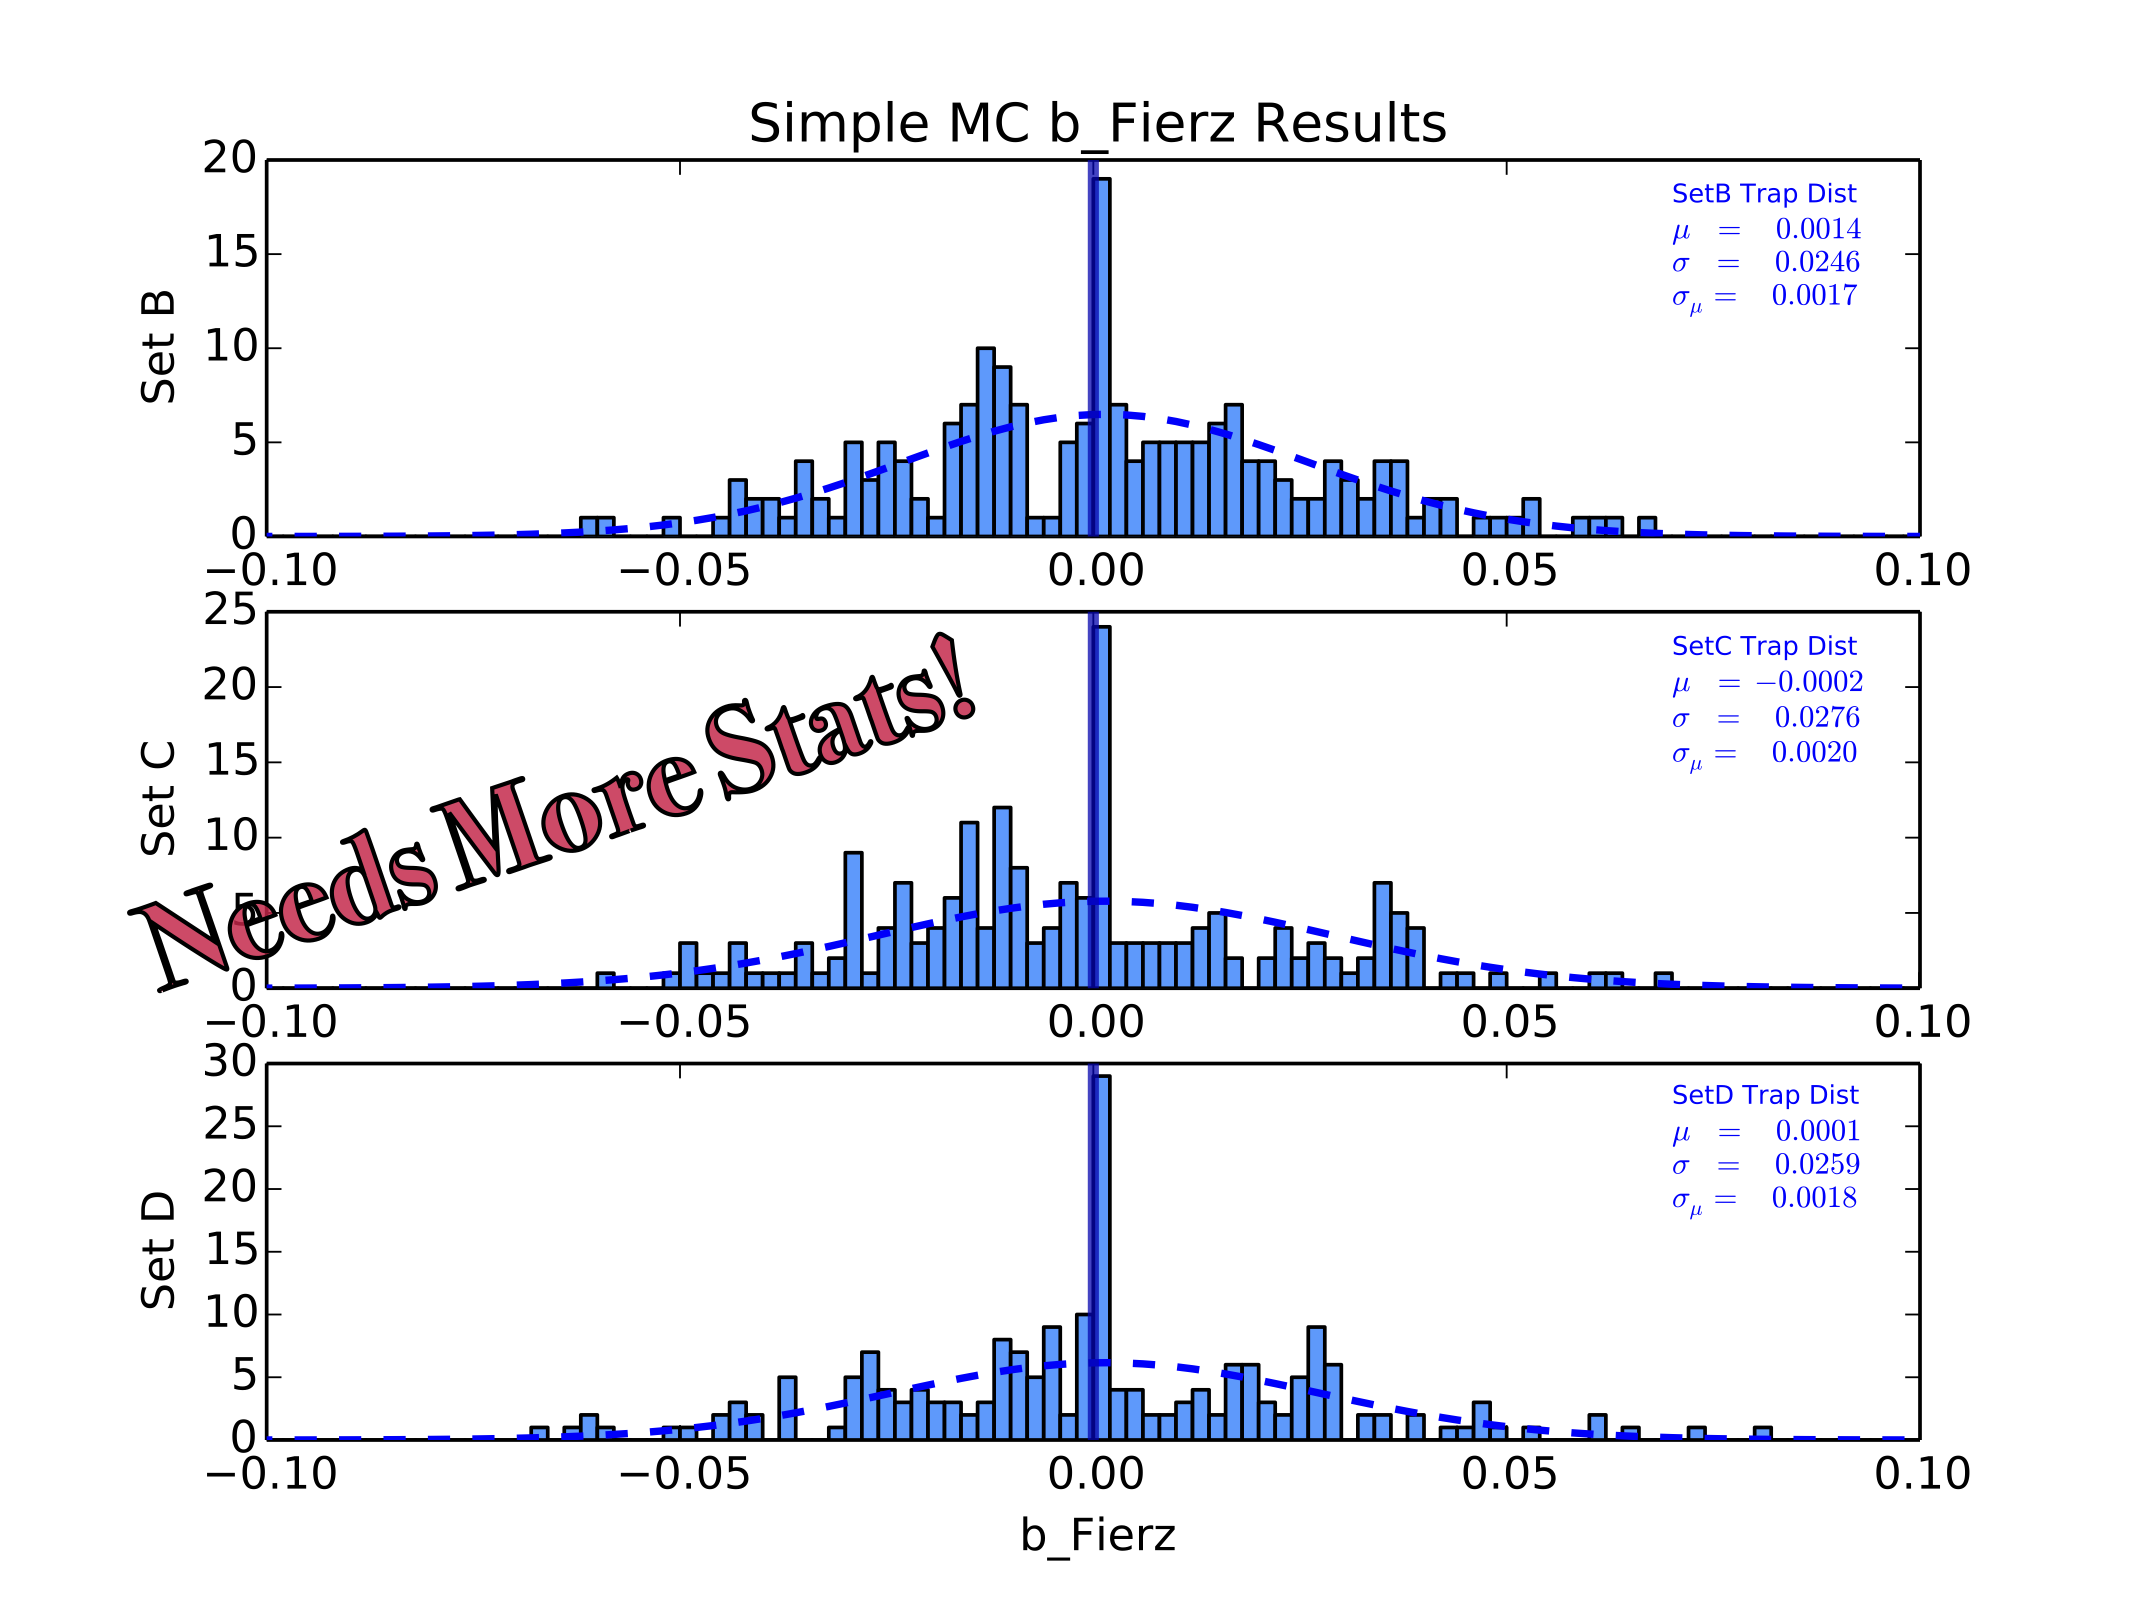
\includegraphics[width=.999\linewidth]
    	{Figures/Position_Err_bFierz_prelim.png}
    	\caption[$\bFierz$ Position Error]{Estimated uncertainty in $\bFierz$ resulting from uncertainty and variation in the cloud parameters.  Evaluated by the lineshape reconstruction method.}		
    	\label{fig:bFierz_position_err}
		\end{figure}

	
	\subsection{The low-energy tail uncertainty, and what it does}
	Bremsstrahlung.  It does Bremsstrahlung.
	\note[color=jb]{JB:  ``I will write this up better soon."  (I think he already did that)}


%\section{Summary of Data Collected}
%\missingfigure{TBH, the thing that's missing is a table, not a figure.  Needs a table full of systematic errors.  And maybe statistical errors?  wev.}
%\note{Needs an error budget table.  Because of course it fucking does.}

